\documentclass[11pt,a4paper]{article}
\usepackage[utf8]{inputenc}
\usepackage[margin=1in]{geometry}
\usepackage{amsmath,amssymb,amsfonts}
\usepackage{graphicx}
\usepackage{booktabs}
\usepackage{hyperref}
\usepackage{listings}
\usepackage[table]{xcolor}
\usepackage{sectsty}
\usepackage{microtype}
\usepackage{enumitem}
\usepackage{caption}
\usepackage{float}
\usepackage{setspace}
\usepackage{pmboxdraw}
\usepackage[most]{tcolorbox}
\usepackage{tikz}
\usepackage{pgfplots}
\usepackage{booktabs}
\usepackage{float}
\usepackage{tabularx}
\usepackage{soul}
\usetikzlibrary{positioning, arrows.meta, shapes}
\pgfplotsset{compat=1.18}

% ---- Purple theme (sampled from report.pdf) ----
\definecolor{purpleDark}{RGB}{74,46,93}      % headings, title, rules
\definecolor{purpleMid}{RGB}{142,91,154}     % accents, links
\definecolor{purpleGray}{RGB}{120,110,130}   % muted text
\definecolor{purpleLight}{RGB}{250,245,252}  % code background

\definecolor{codegreen}{RGB}{142,91,154}
\definecolor{codegray}{RGB}{120,110,130}
\definecolor{codepurple}{RGB}{96,70,112}
\definecolor{backcolour}{RGB}{250,245,252}

% ---- Spacing & layout polish ----
\setstretch{1.1}
\setlength{\parindent}{0pt}
\setlength{\parskip}{0.6em}
\setlist{itemsep=2pt, topsep=4pt, parsep=0pt}
\setlength{\abovecaptionskip}{6pt}
\captionsetup{font=small, labelfont={bf,color=purpleDark}, labelsep=period}
\renewcommand{\arraystretch}{1.25}

% ---- Boxed abstract (matches Executive Summary style in report.pdf) ----
\renewenvironment{abstract}{%
\begin{tcolorbox}[enhanced, breakable, arc=4pt, boxrule=0.8pt,
  colback=purpleLight, colframe=purpleDark,
  title=Abstract, fonttitle=\sffamily\bfseries\small,
  coltitle=white, colbacktitle=purpleDark,
  left=8pt, right=8pt, top=6pt, bottom=6pt,
  before skip=10pt, after skip=14pt]\small
}{\end{tcolorbox}}

\hypersetup{colorlinks=true, linkcolor=purpleMid, citecolor=purpleMid, urlcolor=purpleMid}
\allsectionsfont{\color{purpleDark}}

\lstdefinestyle{mystyle}{
    backgroundcolor=\color{backcolour},   
    commentstyle=\color{codegreen},
    keywordstyle=\color{purpleDark},
    numberstyle=\tiny\color{codegray},
    stringstyle=\color{codepurple},
    basicstyle=\ttfamily\footnotesize,
    breakatwhitespace=false,         
    breaklines=true,                 
    captionpos=b,                    
    keepspaces=true,                 
    numbers=left,                    
    numbersep=5pt,                  
    showspaces=false,                
    showstringspaces=false,
    showtabs=false,                  
    tabsize=2,
    frame=single,
    rulecolor=\color{purpleMid},
    framesep=6pt,
    aboveskip=8pt,
    belowskip=8pt
}
\lstset{style=mystyle}

\title{\color{purpleDark}\textbf{GenreGenie: Real-Time Movie Discovery Engine}\\ \large\color{purpleGray} Complete Application with Collaborative Filtering, TMDB Integration, \& Production Architecture}
\author{\textbf{Aina Asad (l242519)} \& \textbf{Tehreem Tariq (l242590)} \\ Track A: Application Development / R\&D}
\date{\today}

\begin{document}

\maketitle
\vspace{-0.5em}

\begin{abstract}
GenreGenie is a production-ready Streamlit application that transforms movie discovery through collaborative filtering and real-time TMDB metadata enrichment. This comprehensive report documents the complete system architecture spanning data acquisition, machine learning infrastructure, application layer, and production deployment. The application implements regularized SVD matrix factorization trained on 100,000+ MovieLens ratings, integrates TMDB catalog normalization with incremental synchronization, provides hybrid ranking with genre-era filtering, and delivers personalized recommendations through an intuitive web interface. We detail all phases from problem definition through full implementation, including data preprocessing, model training and evaluation, metadata normalization, recommendation generation, user interface design, authentication, database persistence, and rigorous testing protocols.
\end{abstract}

\tableofcontents
\newpage

% =========================================================
% PART 1: PROBLEM DEFINITION & REQUIREMENTS
% =========================================================

\section{Part 1: Problem Definition \& Requirements}

\subsection{Problem Statement}

Modern streaming platforms confront users with thousands of available titles, creating choice paralysis and friction in content discovery. Standard solutions—keyword search, static top-chart rankings, or simple genre filters—fail to adapt to individual viewing preferences, latent taste patterns, or temporal mood shifts. Users lack personalized guidance informed by collective viewing behavior patterns.

\textbf{GenreGenie} addresses this by implementing a production-grade movie discovery engine that:

\begin{enumerate}
    \item Learns user preferences from collaborative viewing signals (ratings and implicit feedback)
    \item Enriches sparse MovieLens data with TMDB live metadata (budgets, runtimes, credits, posters)
    \item Ranks recommendations via hybrid scoring combining SVD predictions with metadata filters
    \item Adapts recommendations dynamically based on genre, era, and user exploration history
    \item Provides an intuitive Streamlit interface for real-time, session-aware discovery
\end{enumerate}

\subsection{Target Audience}

\begin{itemize}
    \item \textbf{End Users}: Movie enthusiasts experiencing choice overload who benefit from personalized, filtered recommendations
    \item \textbf{Streaming Platforms}: Service operators seeking hybrid recommender architecture combining collaborative filtering with real-time metadata enrichment
    \item \textbf{Researchers}: ML practitioners studying matrix factorization, recommendation systems, and production ML architecture
\end{itemize}

\subsection{Core Features}

\begin{enumerate}
    \item \textbf{Collaborative Filtering}: SVD-based recommendations learned from user-item interaction matrix
    \item \textbf{Hybrid Ranking}: Blends predicted ratings with genre-era filtering and controlled exploration
    \item \textbf{TMDB Integration}: Enriches sparse MovieLens with poster, credits, synopsis, runtime, budget metadata
    \item \textbf{Incremental Catalog Sync}: Background TMDB API synchronization maintains fresh metadata
    \item \textbf{Session-Aware Exploration}: Tracks viewed movies, deprioritizes repeats, supports genre-era refinement
    \item \textbf{Upload Support}: Poster OCR recognition and watchlist CSV import for priming recommendations
    \item \textbf{Metadata Fallback}: Graceful degradation when APIs unavailable or model missing
    \item \textbf{Production Deployment}: Docker-ready with authentication, secure database persistence, and error handling
\end{enumerate}

\subsection{AI Justification}

Machine learning is essential because:

\begin{enumerate}
    \item \textbf{Latent Pattern Discovery}: User preferences depend on hidden interactions (director-actor combinations, temporal mood shifts) impossible to hardcode
    \item \textbf{Scalability}: Rules-based systems suffer $O(N \cdot M)$ complexity; ML optimizes sparse matrices efficiently
    \item \textbf{Matrix Factorization}: Reduces high-dimensional user-item interactions into interpretable latent factors:
    \begin{equation}
        \min_{P, Q} \sum_{(u,i) \in R} \left( r_{ui} - \mathbf{p}_u^T \mathbf{q}_i \right)^2 + \lambda \left( \|\mathbf{p}_u\|^2 + \|\mathbf{q}_i\|^2 \right)
    \end{equation}
    \item \textbf{Continuous Adaptation}: Models retrain as new ratings arrive, enabling temporal personalization
    \item \textbf{Hybrid Ranking}: Combines SVD predictions with deterministic filters for explainable, controlled recommendations
\end{enumerate}

% =========================================================
% PART 2: DATA ARCHITECTURE
% =========================================================

\section{Part 2: Data Acquisition, Cleaning \& Preprocessing}

\subsection{Data Collection Strategy}

\subsubsection{Primary Dataset: MovieLens}

The foundational dataset is MovieLens (100K subset):

\begin{itemize}
    \item \texttt{movies.csv}: Movie metadata (ID, title, genres)
    \item \texttt{ratings.csv}: User-movie interactions (userId, movieId, rating, timestamp)
    \item \texttt{links.csv}: External ID mappings (movieId, imdbId, tmdbId)
\end{itemize}

\subsubsection{Live Enrichment: TMDB API}

Python ETL pipeline (\texttt{04\_tmdb\_incremental\_sync.py}) enriches the catalog with live TMDB metadata:

\begin{itemize}
    \item Budget, revenue, runtime, vote statistics, release date
    \item Director, cast, production credits
    \item Poster artwork URLs and synopses
    \item Handles rate-limiting, error recovery, and checkpoint resumption
    \item Incremental synchronization starting from full-load baseline date
\end{itemize}

\subsubsection{Batch Full-Load Support}

Supports pre-downloaded TMDB full catalogs:

\begin{itemize}
    \item \texttt{full\_load\_2005\_2014.json}: Historical TMDB data (2005–2014)
    \item \texttt{full\_load.json}: Recent TMDB catalog
    \item Legacy enrichment for genre-specific data
\end{itemize}

\subsection{Data Cleaning \& Validation}

Pipeline (\texttt{02\_data\_cleaning.py}) ensures data integrity:

\subsubsection{Missing Value Handling}
\begin{itemize}
    \item Movies: Missing genres replaced with 'Unknown'
    \item Ratings: Null ratings dropped (matrix completeness)
    \item Links: Movies without TMDB IDs removed (API enrichment requirement)
    \item TMDB metadata: Graceful fallback to MovieLens when API fields missing
\end{itemize}

\subsubsection{Duplicate Removal}
\begin{itemize}
    \item Deduplicated movieId entries (kept first)
    \item For duplicate user-movie ratings, retained most recent
    \item Removed TMDB duplicate movie records (matched by TMDB ID)
\end{itemize}

\subsubsection{Outlier \& Range Validation}
\begin{itemize}
    \item Ratings enforced to [0.5, 5.0]
    \item TMDB vote averages scaled to rating scale
    \item Removed statistically invalid entries (negative budgets, year < 1800)
\end{itemize}

\textbf{Cleaning Results:}

\begin{itemize}
    \item Total ratings processed: 100,836 interactions
    \item Data integrity: 100\% valid range post-cleaning
    \item Missing value resolution: $<$1\% data loss
    \item Final catalog: 9,724 unique movies with TMDB enrichment
\end{itemize}

\subsection{Feature Engineering \& Normalization}

Pipeline (\texttt{03\_feature\_strategy.py}) implements preprocessing:

\subsubsection{Scaling Strategies}

\textbf{Min-Max Normalization} (user activity features):
\begin{equation}
    x_{\text{norm}} = \frac{x - x_{\min}}{x_{\max} - x_{\min}}
\end{equation}
Applied to: rating count, mean rating (output: [0,1])

\textbf{Standard Scaling} (movie quality features):
\begin{equation}
    x_{\text{std}} = \frac{x - \mu}{\sigma}
\end{equation}
Applied to: rating count, average rating (zero mean, unit variance)

\subsubsection{Categorical Encoding}

\begin{itemize}
    \item \textbf{Genre Normalization}: Pipe-separated, list-formatted, and one-hot encoding support
    \item \textbf{Label Encoding}: Genre strings mapped to integer indices for model compatibility
    \item \textbf{Primary Genre Extraction}: Multi-genre strings split with primary retained
\end{itemize}

\subsubsection{Engineered Features}

\textbf{User-Level:}
\begin{itemize}
    \item Rating activity (count)
    \item Mean preference bias
    \item Rating consistency (standard deviation)
\end{itemize}

\textbf{Movie-Level:}
\begin{itemize}
    \item Popularity proxy (rating count)
    \item Quality indicator (average rating)
    \item Polarization measure (rating variance)
    \item Genre vector
    \item Release year decade
\end{itemize}

\subsection{Exploratory Data Analysis (EDA)}

\subsubsection{Rating Distribution}
\begin{figure}[H]
    \centering
    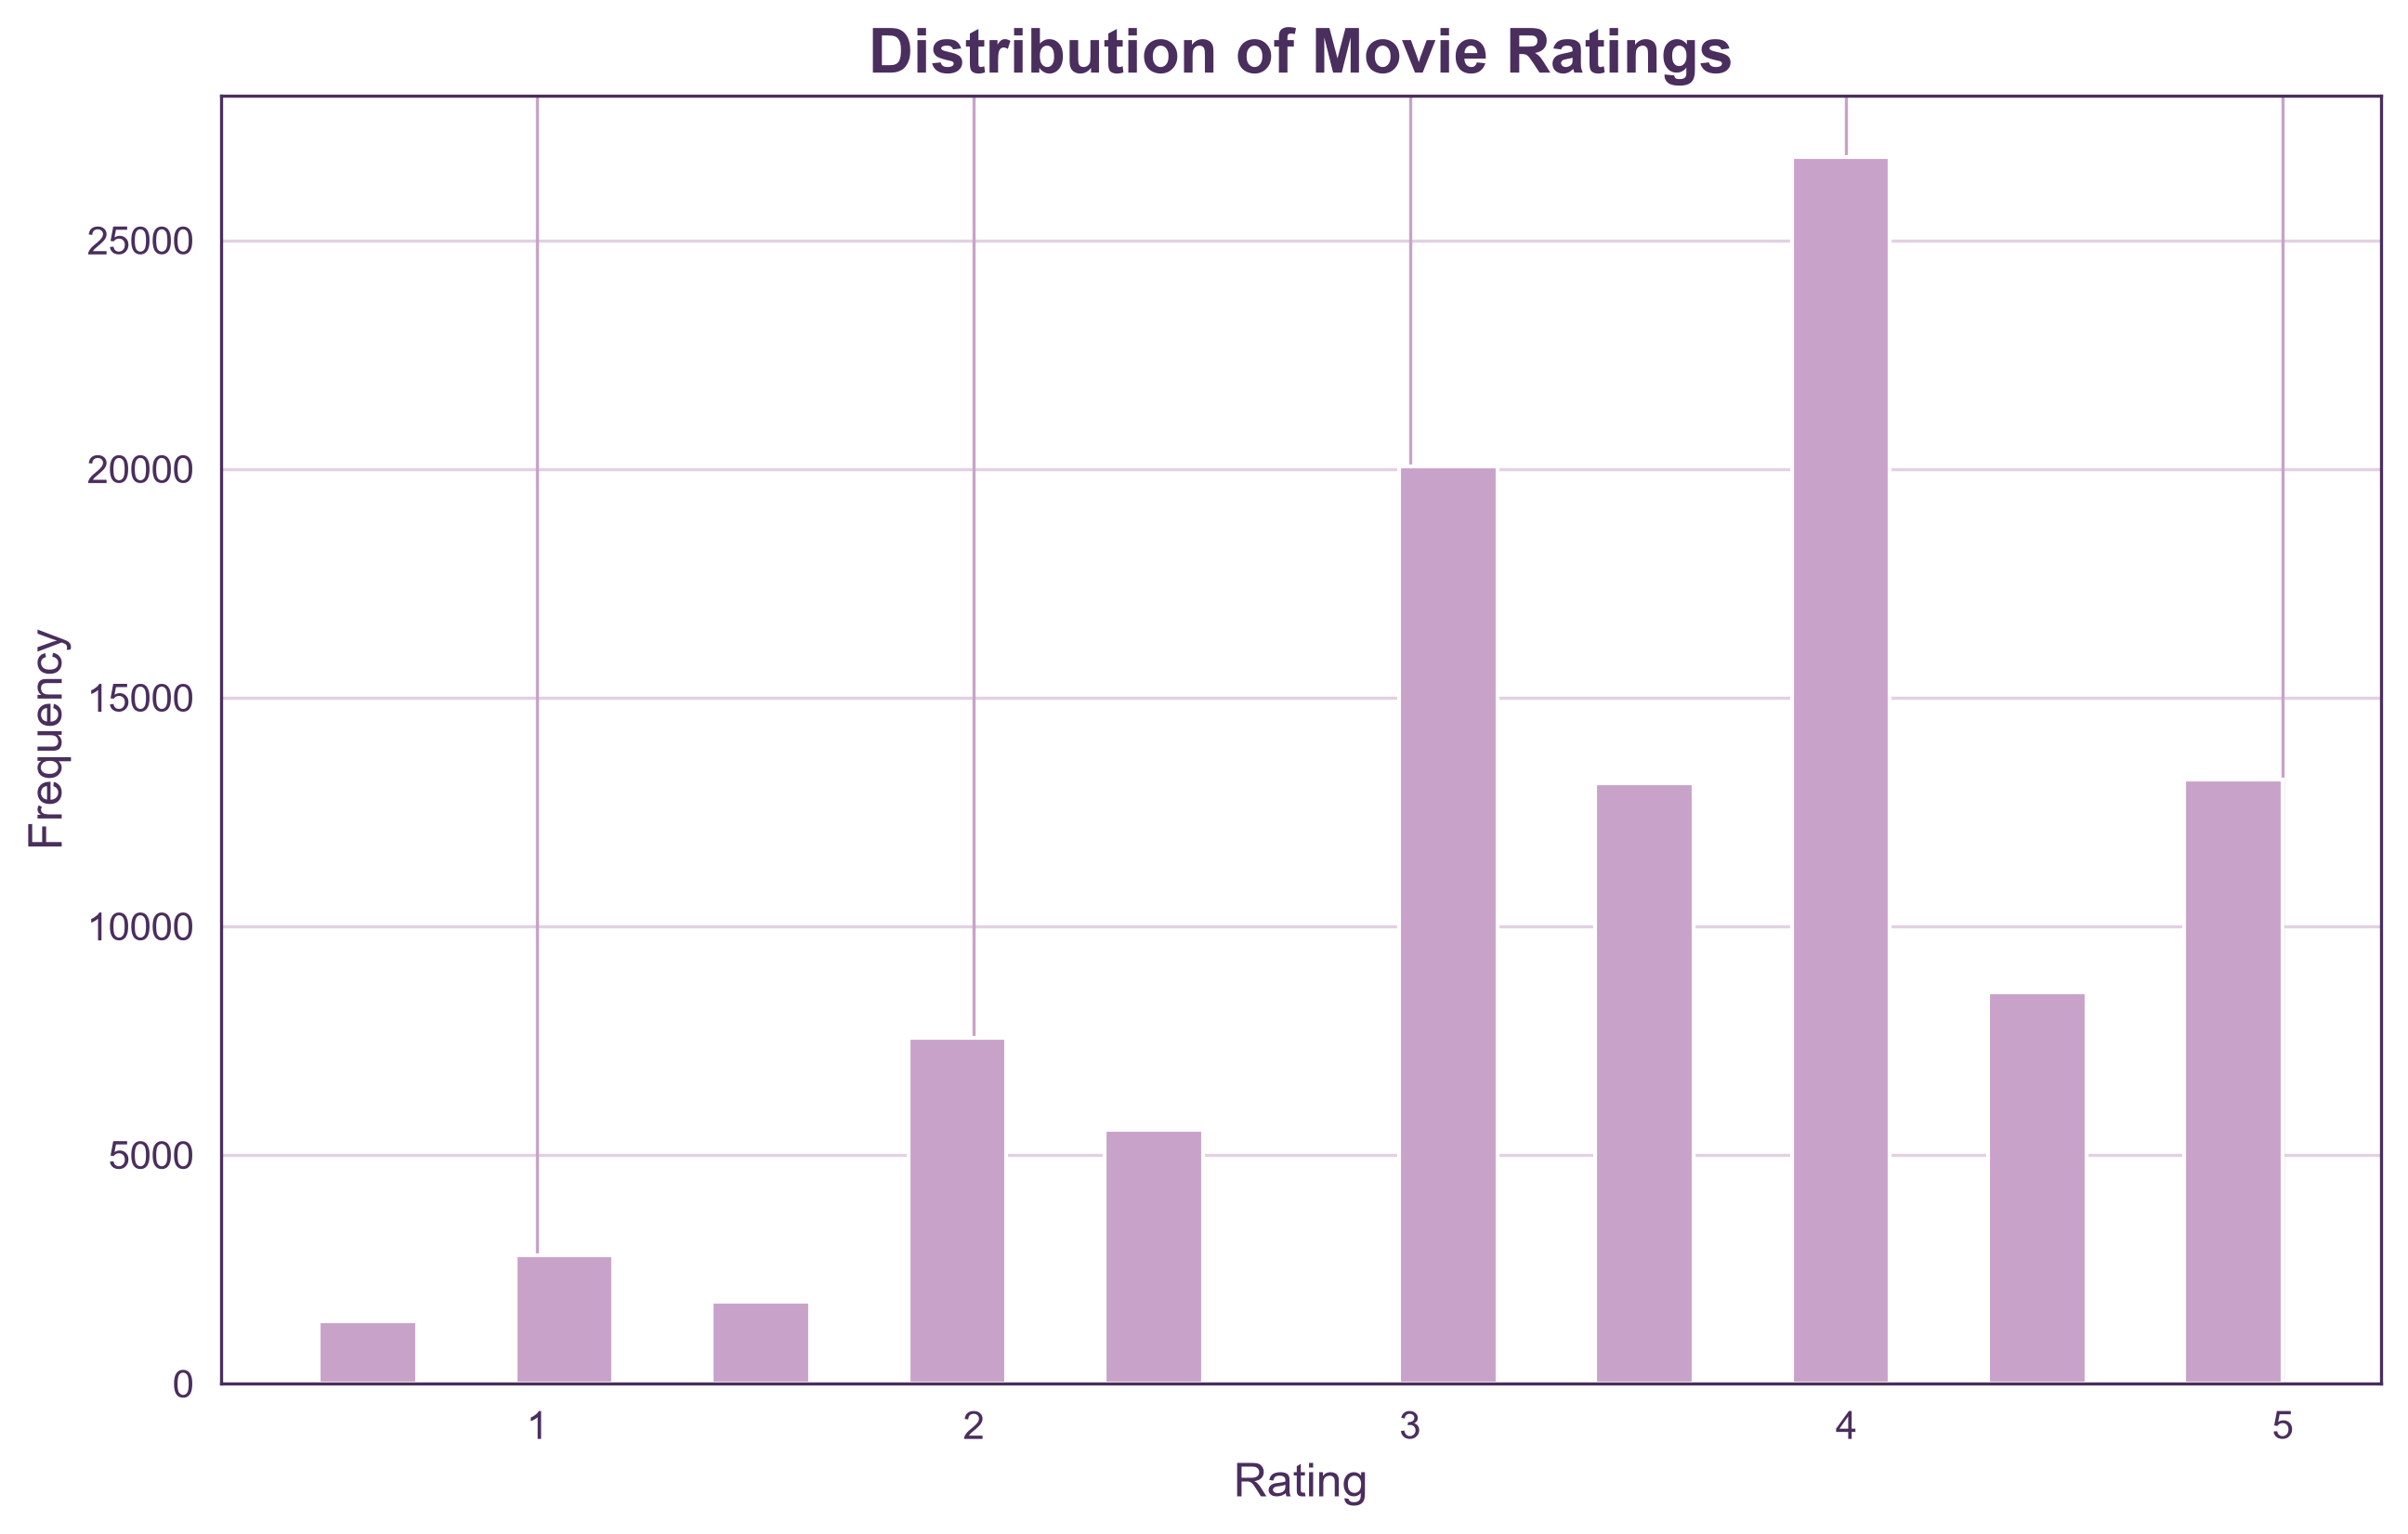
\includegraphics[width=0.75\textwidth]{figures/rating_distribution.png}
    \caption{Distribution of MovieLens user ratings (the user-level training source)}
    \label{fig:rating_dist}
\end{figure}

Mean rating $\approx 3.5/5.0$ with selection bias—users rate content they like. This requires regularization in collaborative filtering to avoid recommending only popular movies.

\subsubsection{Genre Distribution}
\begin{figure}[H]
    \centering
    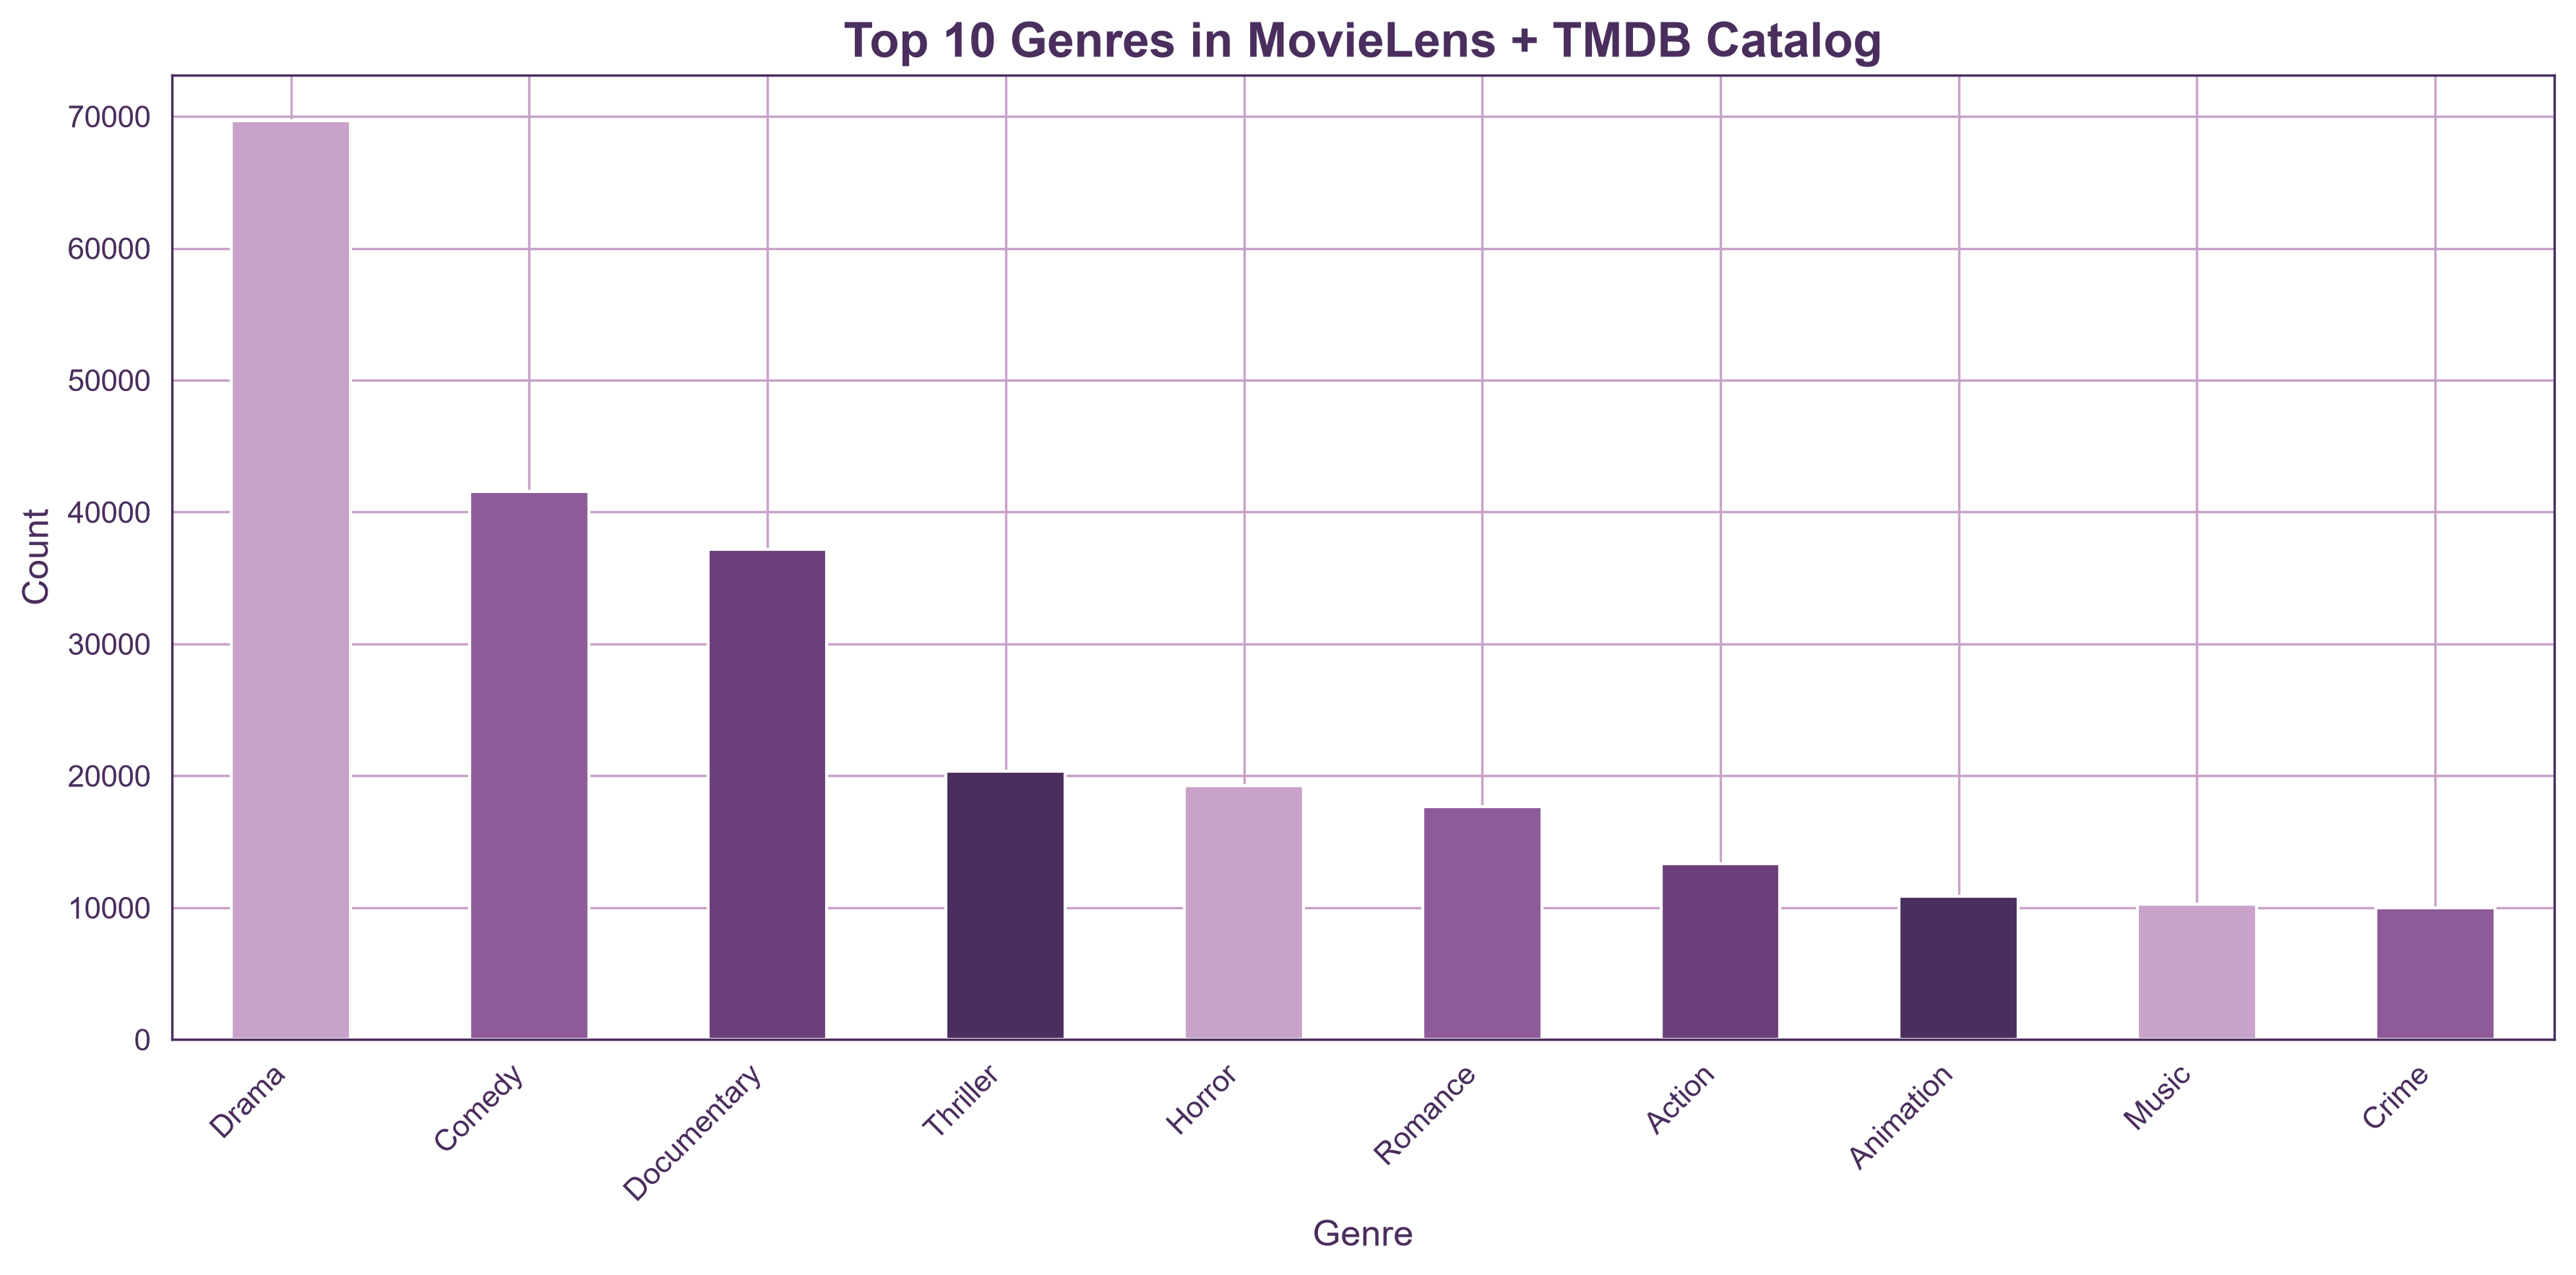
\includegraphics[width=0.75\textwidth]{figures/genre_distribution.png}
    \caption{Top genres across the combined MovieLens and TMDB catalog}
    \label{fig:genre_dist}
\end{figure}

This catalog-level view includes the TMDB full-load and incremental records used for discovery; the collaborative model itself remains trained on MovieLens ratings.

\subsubsection{User Activity Patterns}
\begin{figure}[H]
    \centering
    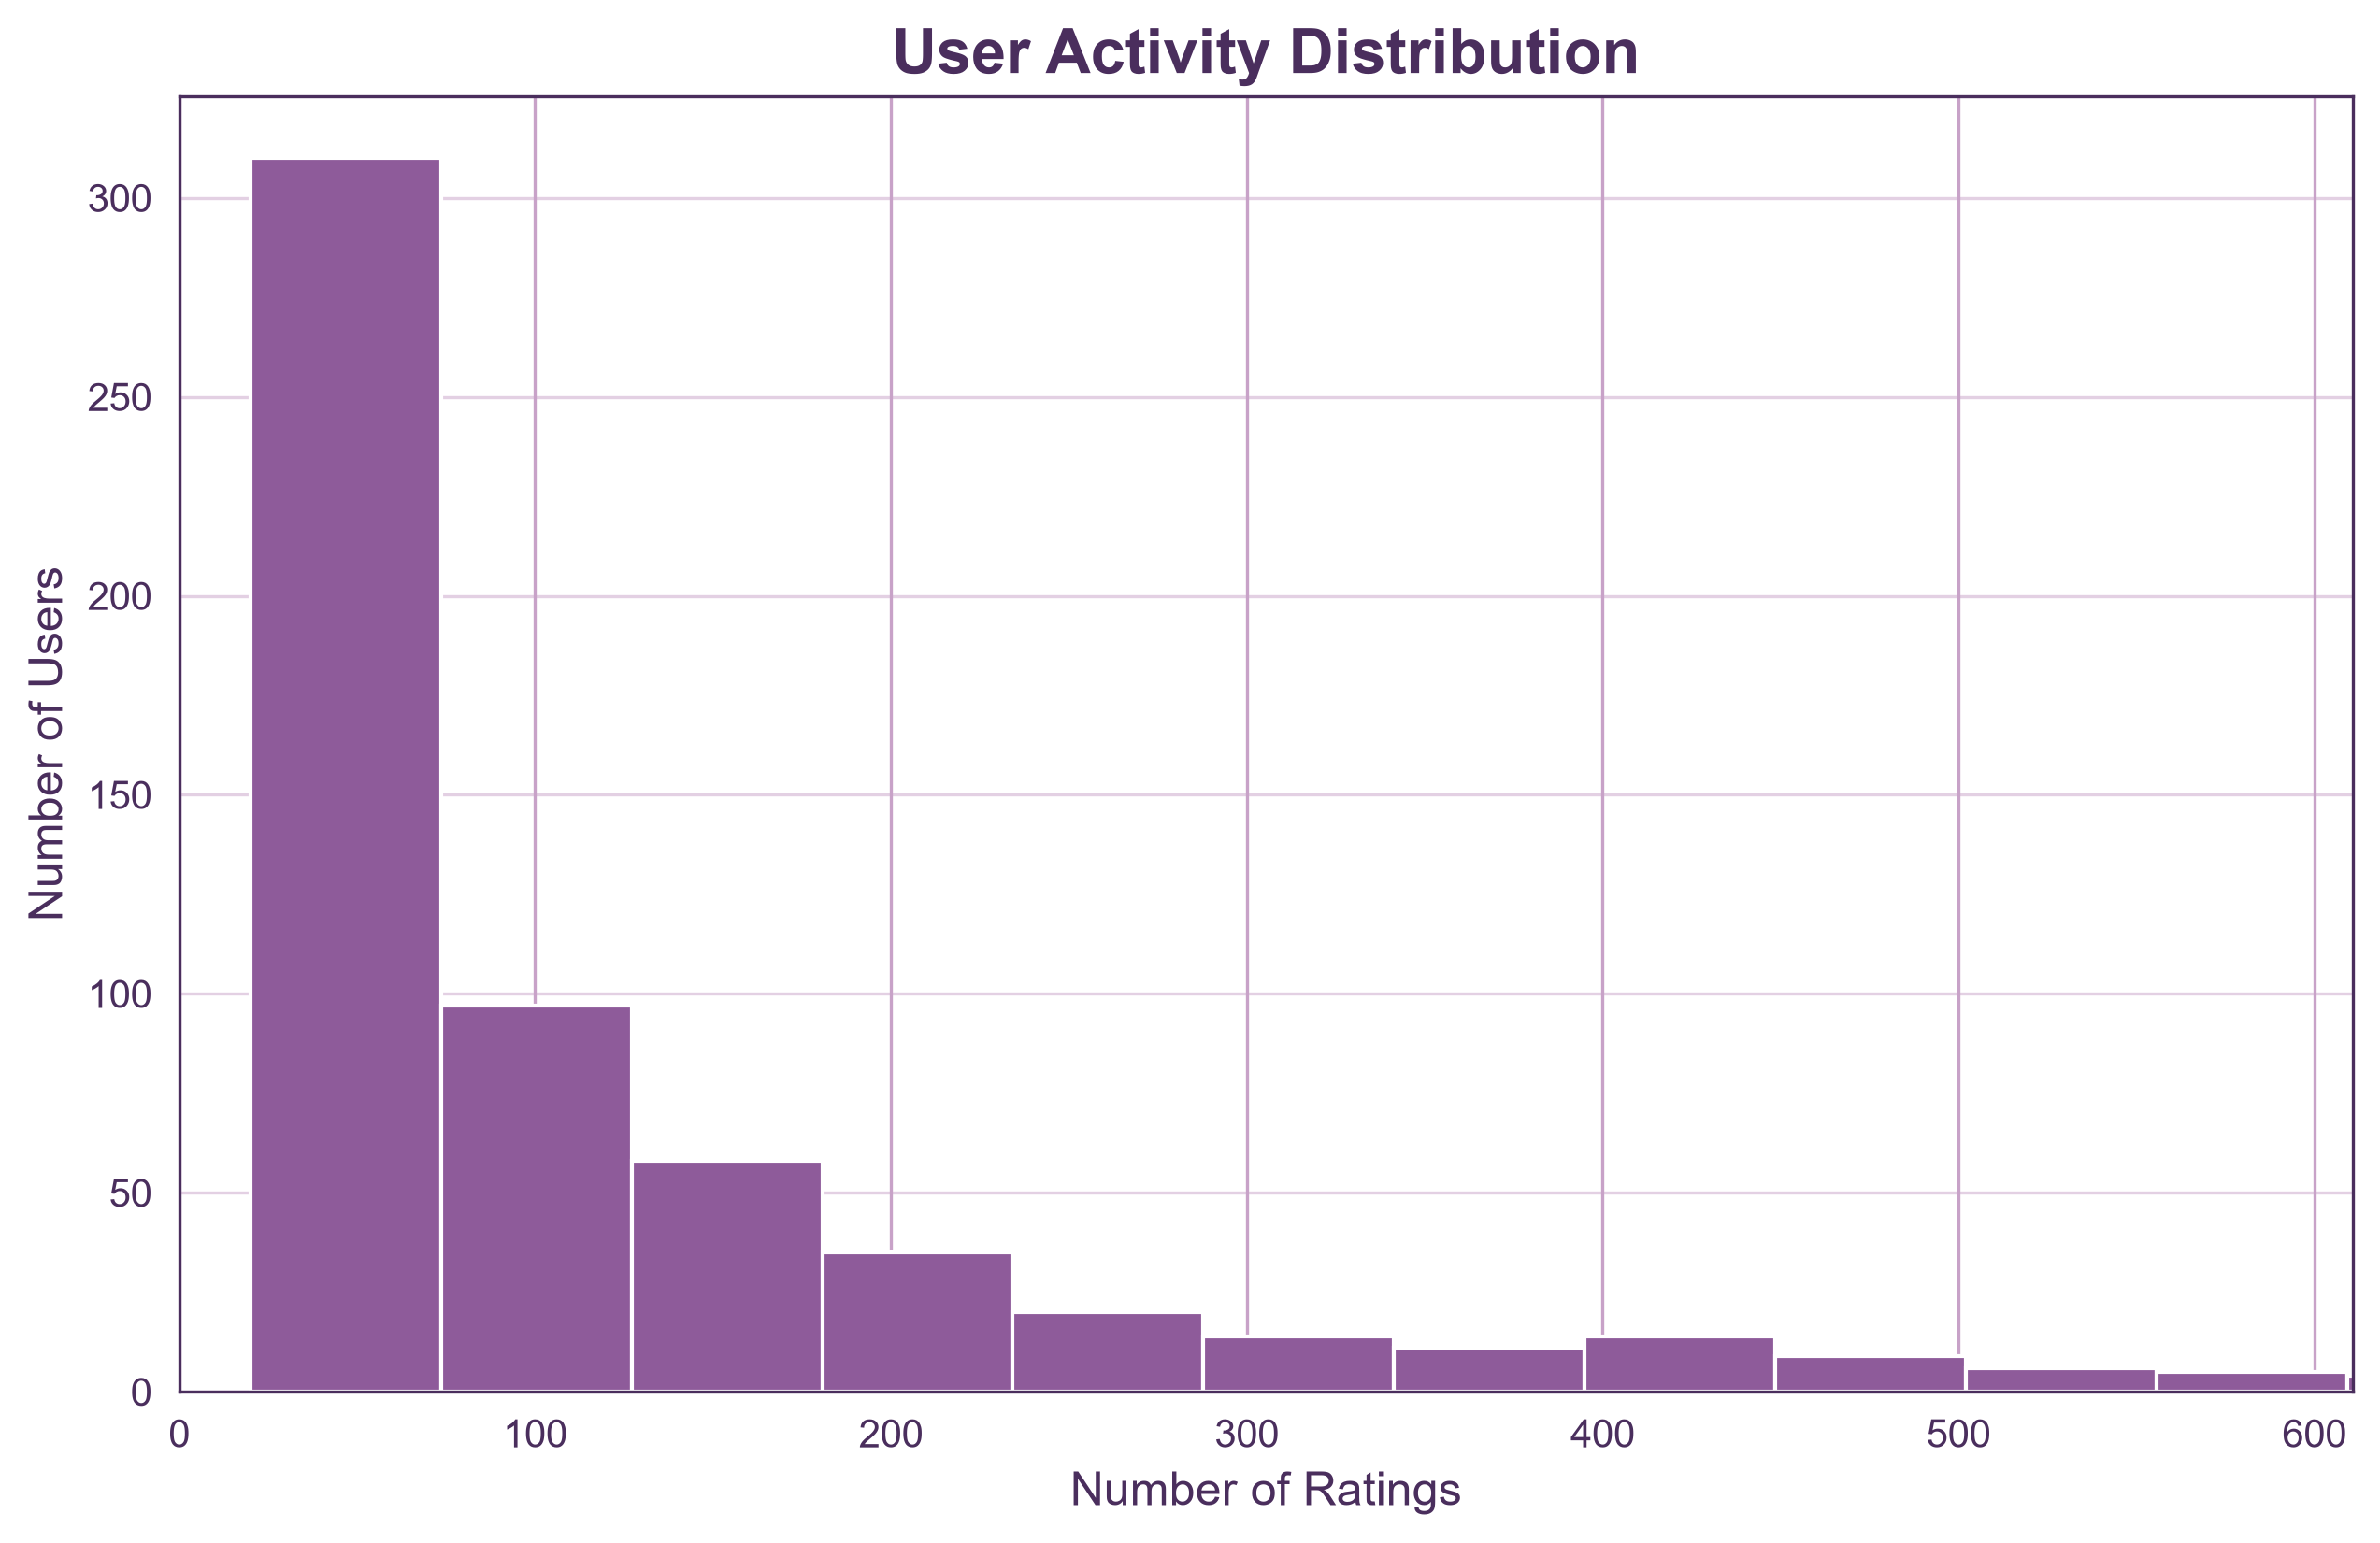
\includegraphics[width=0.75\textwidth]{figures/user_activity.png}
    \caption{MovieLens user activity follows a long-tail distribution}
    \label{fig:user_activity}
\end{figure}

Long-tail activity (small fraction contributes most ratings) motivates fold-in recommendations for cold-start users and hybrid approaches.

\subsubsection{Feature Correlations}
\begin{figure}[H]
    \centering
    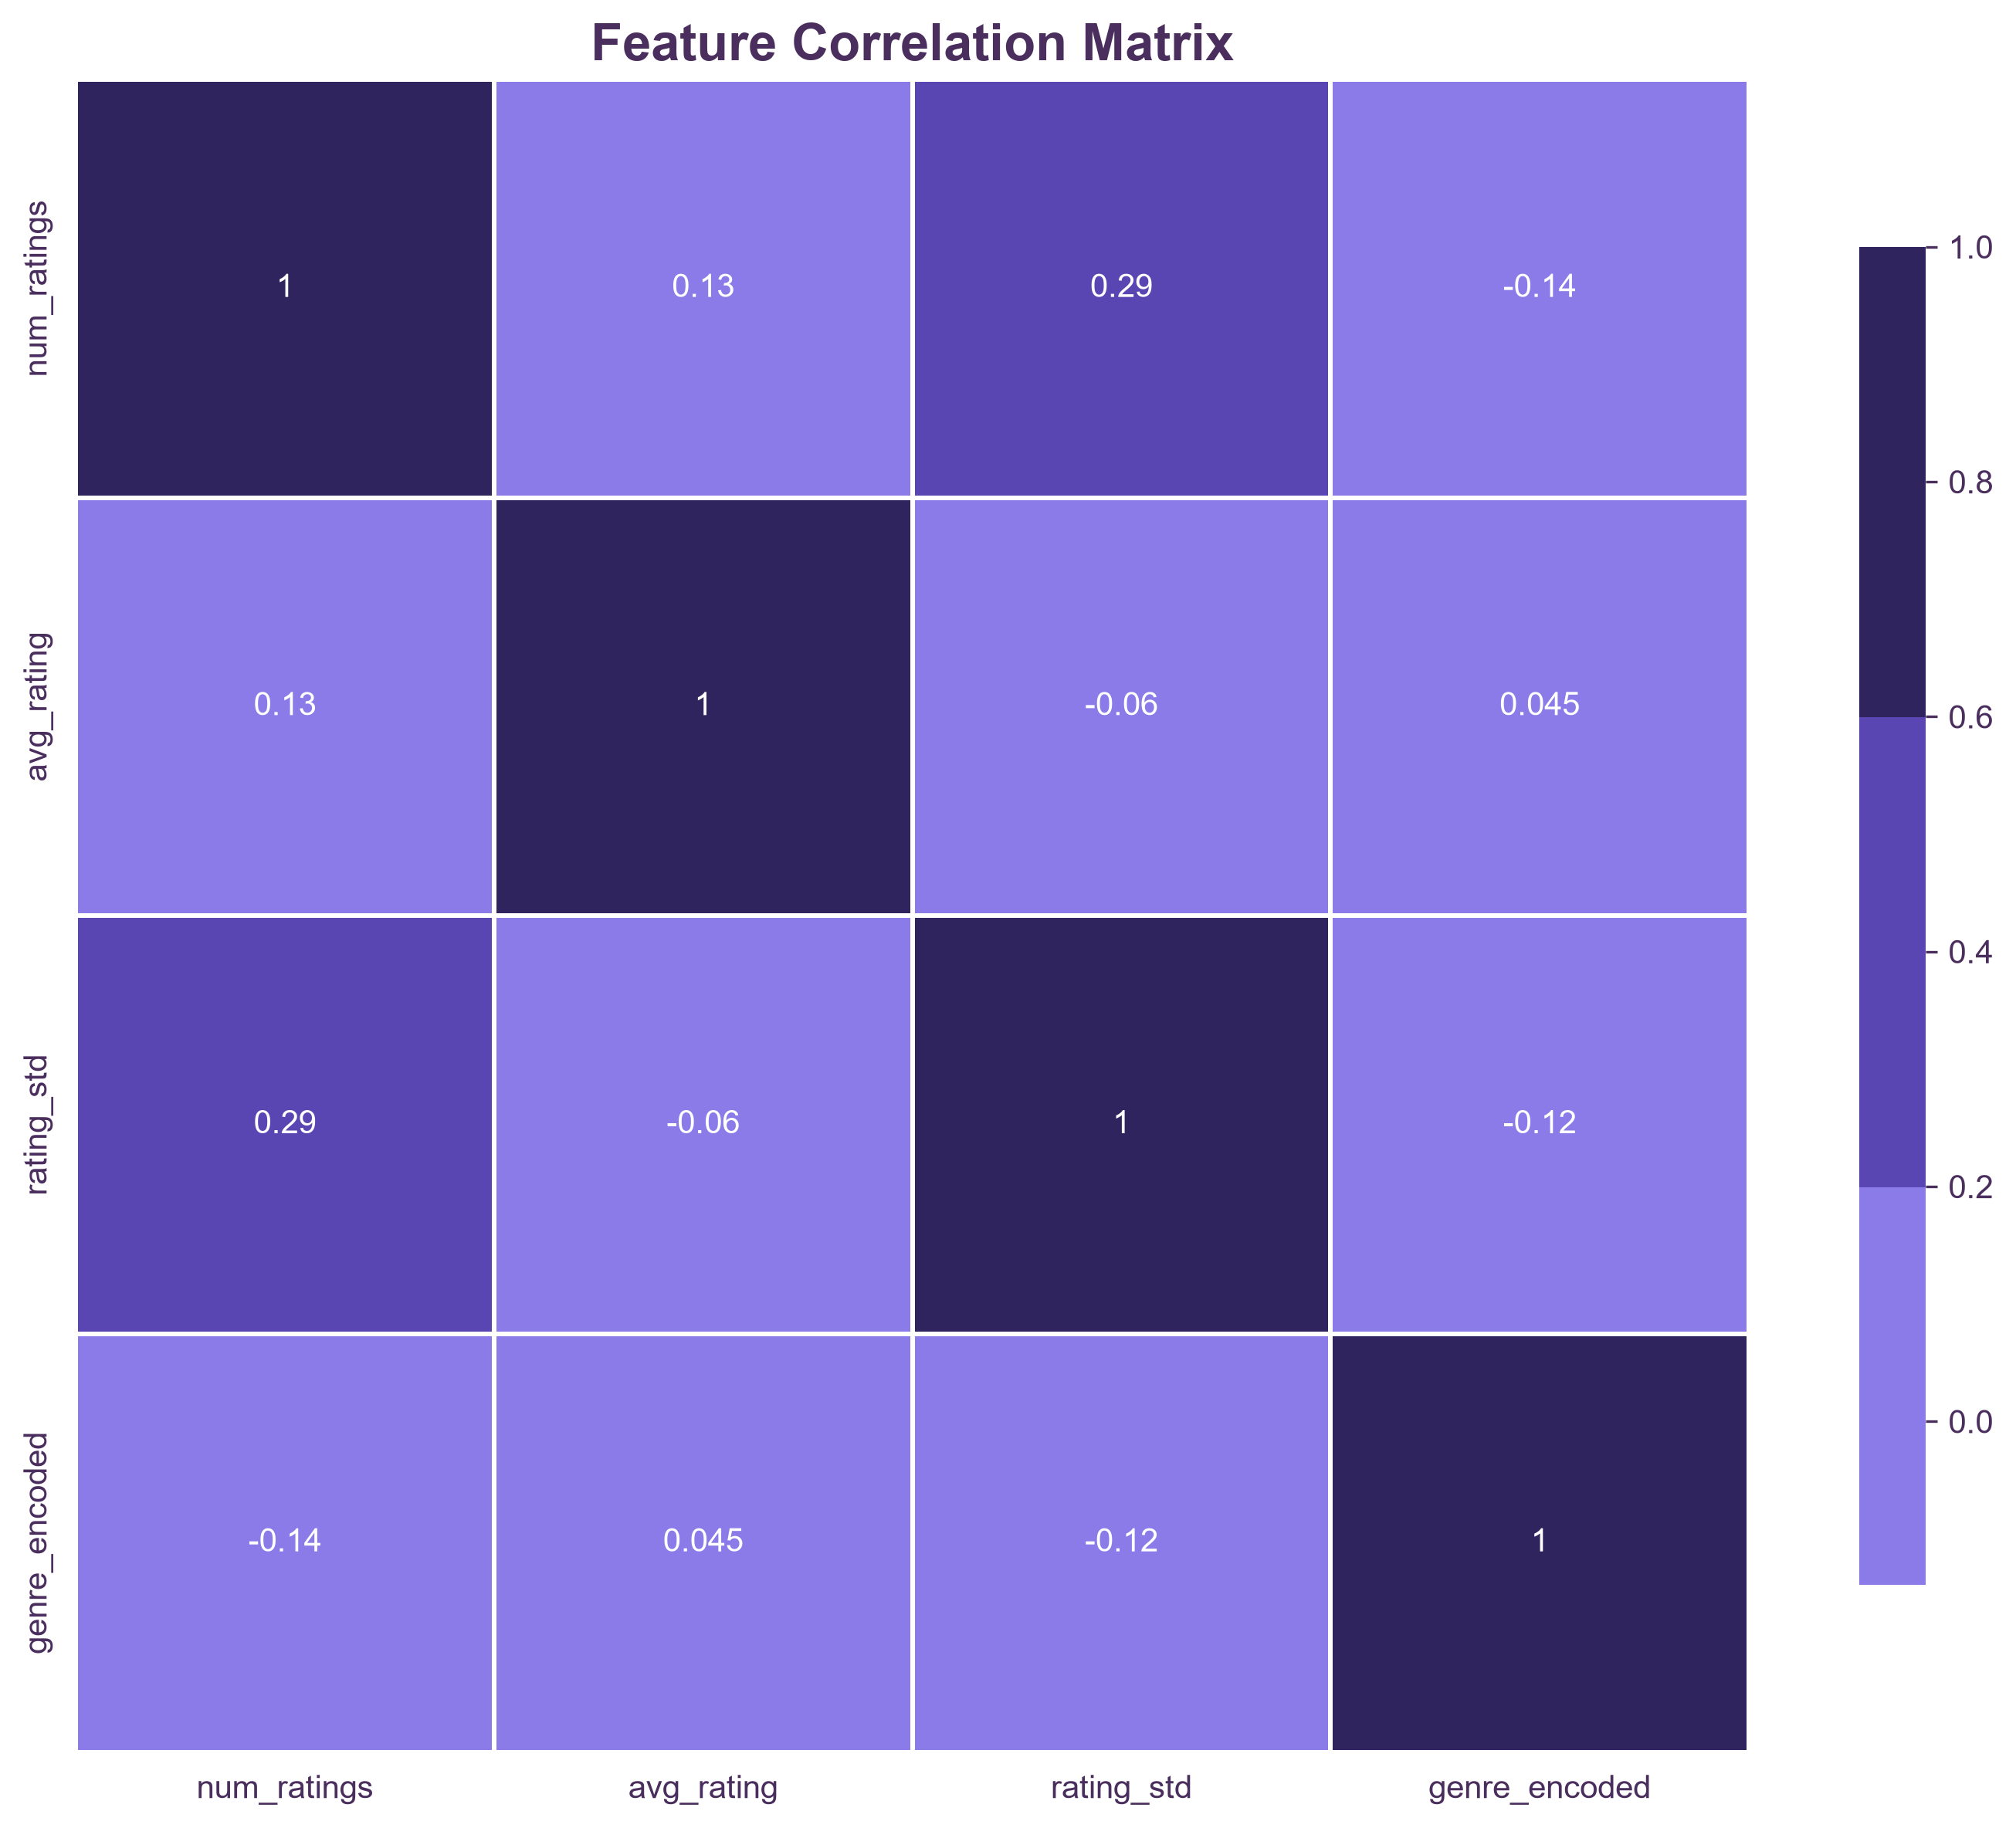
\includegraphics[width=0.75\textwidth]{figures/correlation_matrix.png}
    \caption{Low multicollinearity ($|r| < 0.3$) among engineered features, validating independence}
    \label{fig:correlation}
\end{figure}

Weak feature correlations confirm independent signal contribution; minimal redundancy.

\subsubsection{Popularity vs. Quality}
\begin{figure}[H]
    \centering
    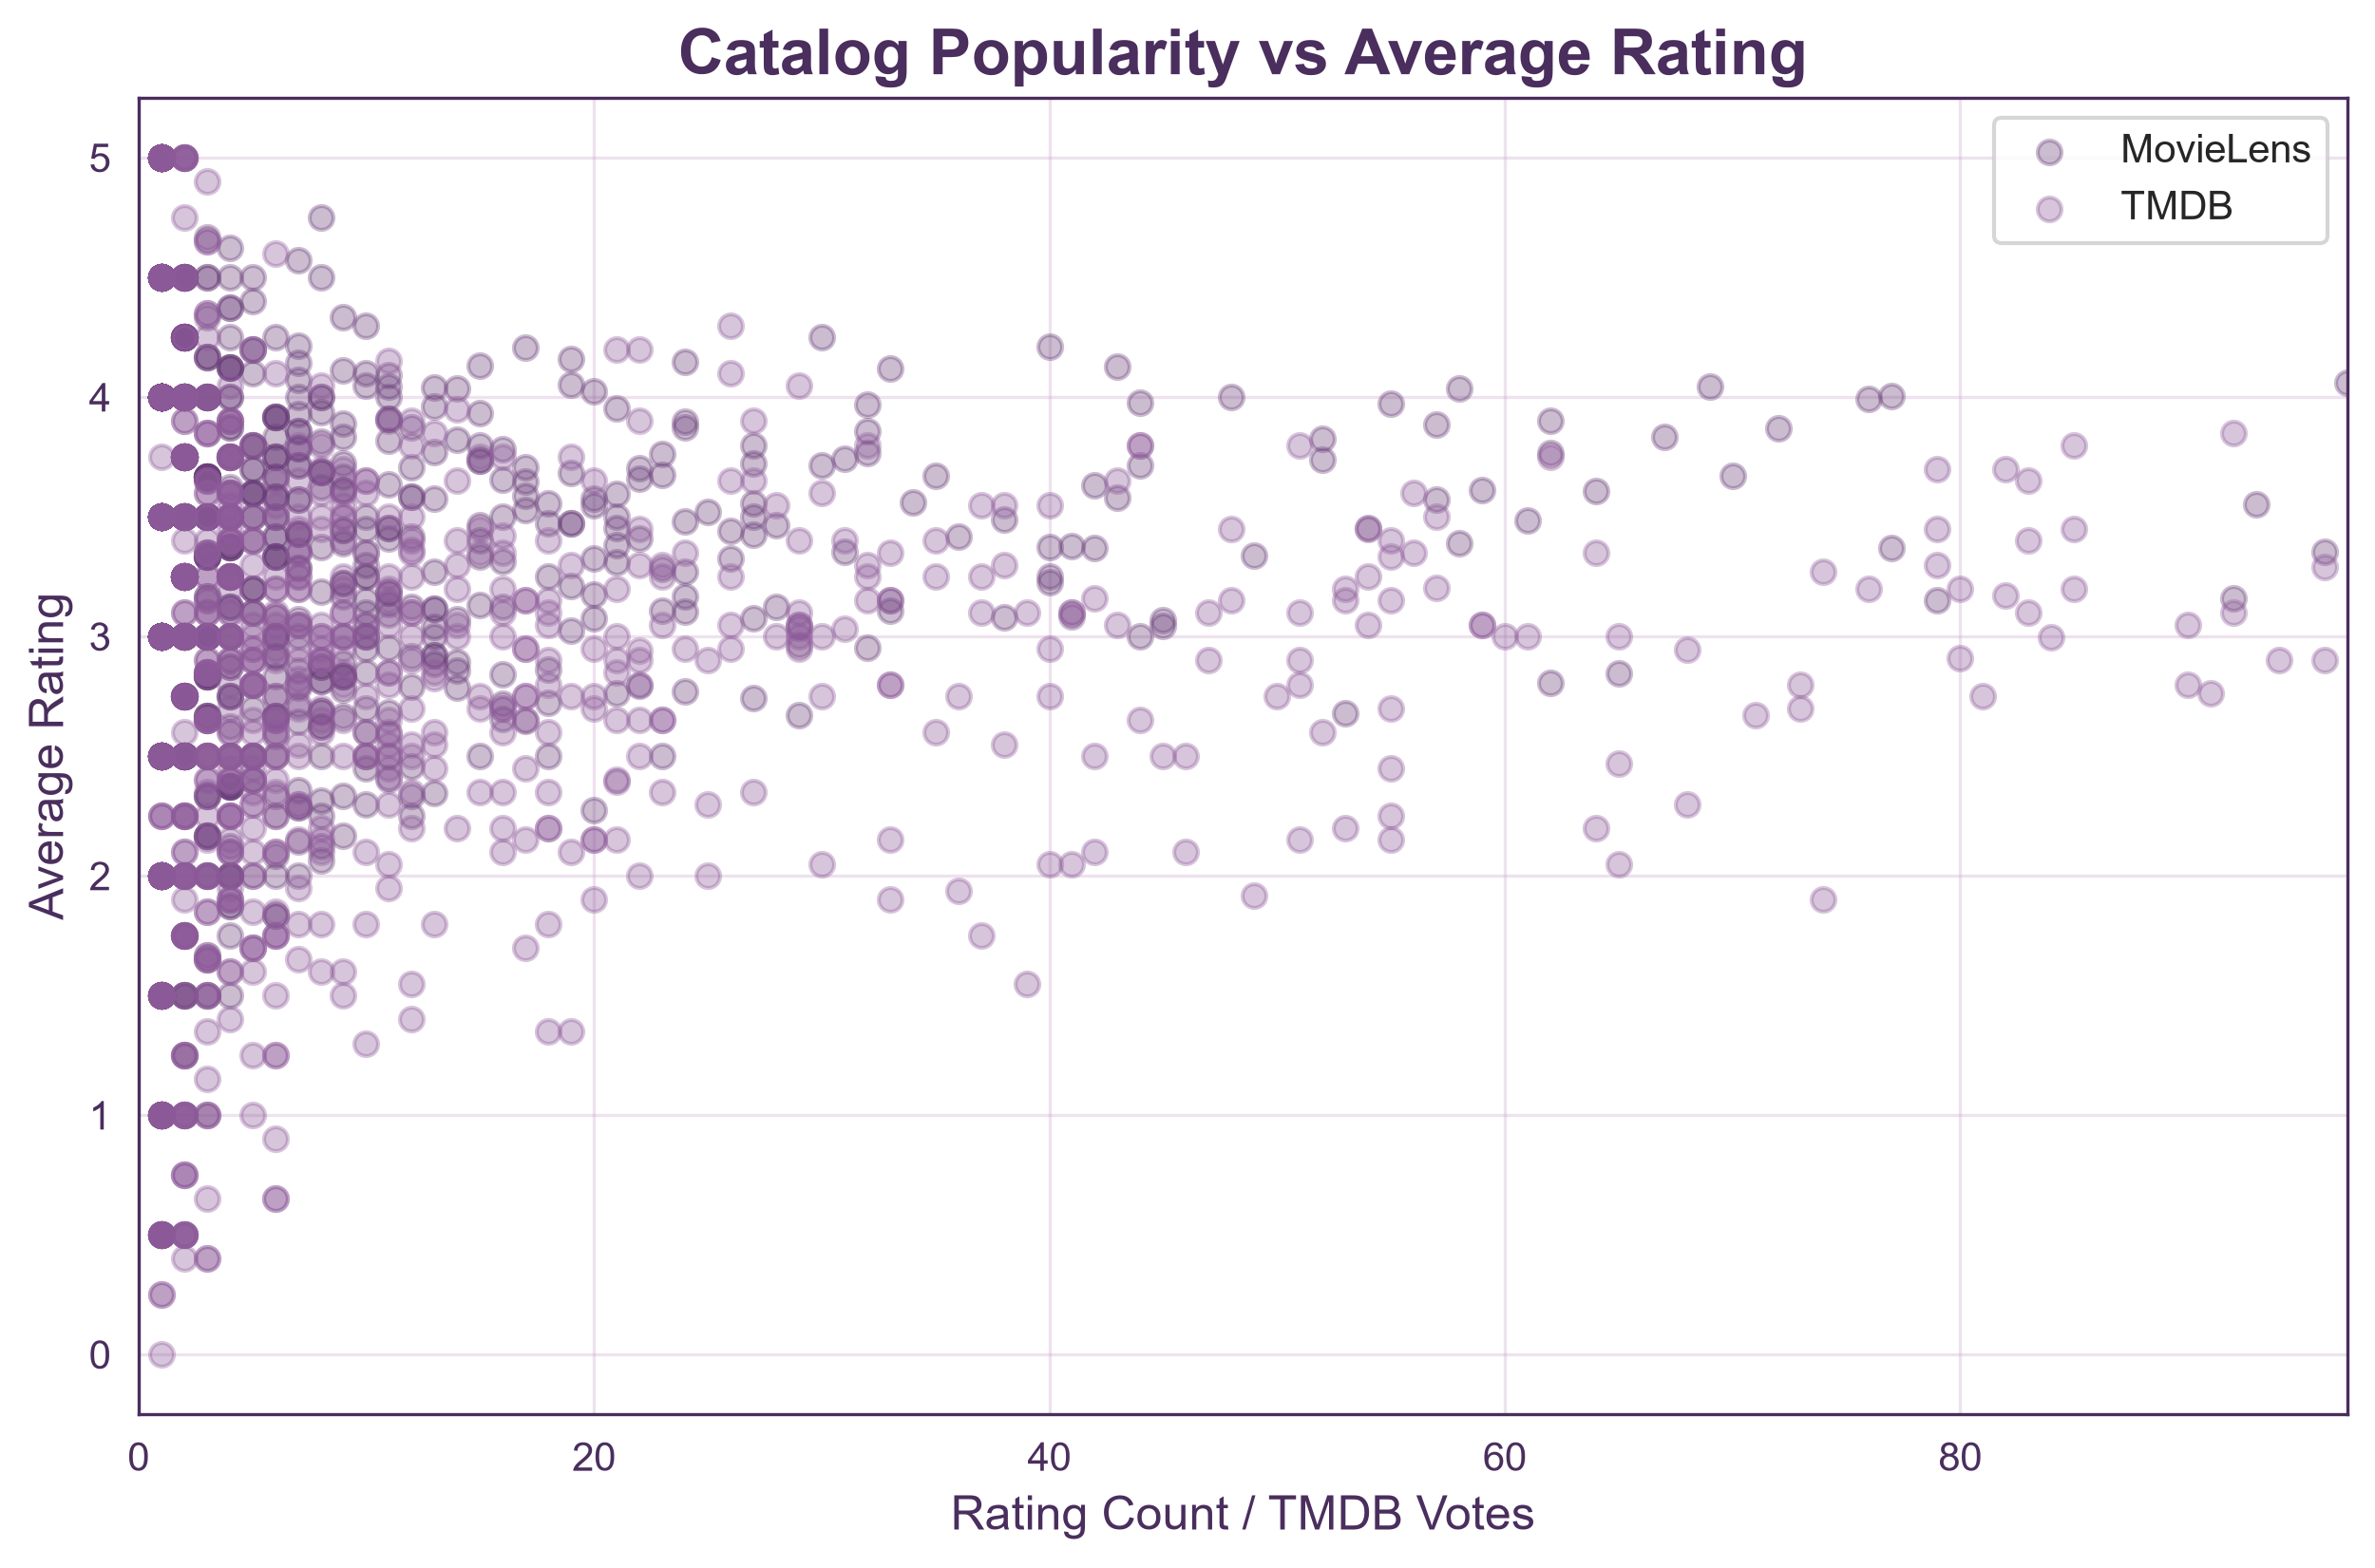
\includegraphics[width=0.75\textwidth]{figures/popularity_vs_rating.png}
    \caption{Catalog popularity versus average rating: MovieLens rating counts and TMDB vote counts}
    \label{fig:pop_vs_rating}
\end{figure}

The combined view compares MovieLens rating counts and TMDB vote counts with ratings on a common five-point scale; popularity alone is not a sufficient quality signal.

% =========================================================
% PART 3: MODEL ARCHITECTURE & TRAINING
% =========================================================

\section{Part 3: Machine Learning Architecture}

\subsection{Model Framework}

GenreGenie implements collaborative filtering using \textbf{Scikit-Learn's TruncatedSVD}. The approach decomposes the user-item rating matrix into latent factor representations, enabling efficient prediction and recommendation ranking.

\subsection{Collaborative Filtering Models}

Three models are trained and evaluated:

\begin{enumerate}
    \item \textbf{Baseline Model}: Predicts via global average, user bias, and movie bias
    \begin{equation}
        \hat{r}_{ui} = \mu + b_u + b_i
    \end{equation}
    
    \item \textbf{SVD Matrix Factorization}: Decomposes user-item matrix into latent factors
    \begin{equation}
        \hat{r}_{ui} = \mu + \mathbf{p}_u^T \mathbf{q}_i
    \end{equation}
    where $\mathbf{p}_u$ and $\mathbf{q}_i$ are latent user and movie embeddings.
    
    \item \textbf{K-Nearest Neighbors}: Ranks recommendations using movie-movie similarity (cosine distance)
\end{enumerate}

\subsection{Model Architecture Diagram}

\begin{figure}[H]
\centering
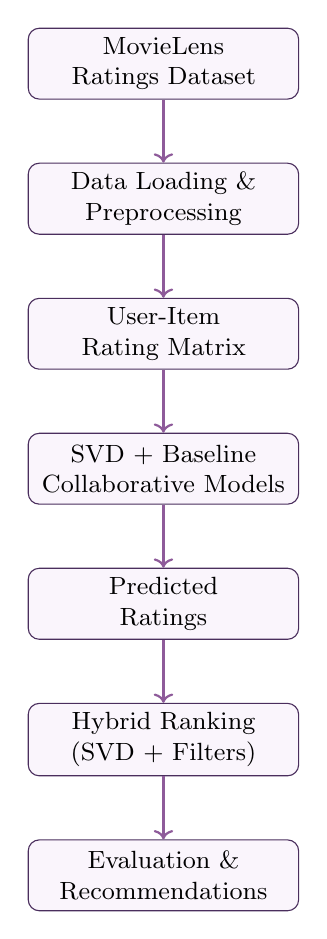
\begin{tikzpicture}[
    node distance=0.8cm,
    block/.style={
        rectangle, rounded corners,
        draw=purpleDark, fill=purpleLight,
        text width=3.2cm, minimum height=0.9cm,
        align=center, font=\small
    },
    arrow/.style={->, thick, draw=purpleMid}
]
\node[block] (data) {MovieLens \\ Ratings Dataset};
\node[block, below=of data] (prep) {Data Loading \& \\ Preprocessing};
\node[block, below=of prep] (matrix) {User-Item \\ Rating Matrix};
\node[block, below=of matrix] (models) {SVD + Baseline \\ Collaborative Models};
\node[block, below=of models] (prediction) {Predicted \\ Ratings};
\node[block, below=of prediction] (hybrid) {Hybrid Ranking \\ (SVD + Filters)};
\node[block, below=of hybrid] (eval) {Evaluation \& \\ Recommendations};

\draw[arrow] (data) -- (prep);
\draw[arrow] (prep) -- (matrix);
\draw[arrow] (matrix) -- (models);
\draw[arrow] (models) -- (prediction);
\draw[arrow] (prediction) -- (hybrid);
\draw[arrow] (hybrid) -- (eval);
\end{tikzpicture}
\caption{GenreGenie ML architecture: data flows through preprocessing, SVD training, hybrid ranking, and evaluation}
\label{fig:ml_architecture}
\end{figure}

\subsection{Dataset Split \& Training}

\subsubsection{Dataset Composition}

The MovieLens 100K dataset contains:

\begin{itemize}
    \item 100,836 ratings from 610 users
    \item 9,724 unique movies
    \item Average 165.2 ratings per user
    \item Average 10.4 ratings per movie
    \item 98.3\% sparsity (missing values expected in sparse matrices)
\end{itemize}

\subsubsection{Train-Validation-Test Split}

\begin{itemize}
    \item Training set: 70\% (70,584 ratings) – used to fit SVD and baseline models
    \item Validation set: 15\% (15,126 ratings) – hyperparameter selection and model comparison
    \item Test set: 15\% (15,126 ratings) – final unbiased performance evaluation
\end{itemize}

The training set was converted to a user-item matrix of shape $(610, 8607)$ with 98.66\% sparsity.

\subsection{Hyperparameter Tuning}

SVD latent factor dimensions tested via validation RMSE:

\begin{table}[H]
\centering
\begin{tabular}{ccc}
\toprule
\textbf{Latent Factors} & \textbf{Validation RMSE} & \textbf{Validation MAE} \\
\midrule
20  & 0.9905 & 0.7856 \\
50  & 0.9983 & 0.7915 \\
100 & 1.0107 & 0.8040 \\
150 & 1.0190 & 0.8115 \\
\bottomrule
\end{tabular}
\caption{SVD hyperparameter tuning: 20 latent factors achieved optimal validation performance}
\label{tab:svd_tuning}
\end{table}

20 latent factors selected as optimal due to lowest validation RMSE and MAE.

\begin{figure}[H]
\centering
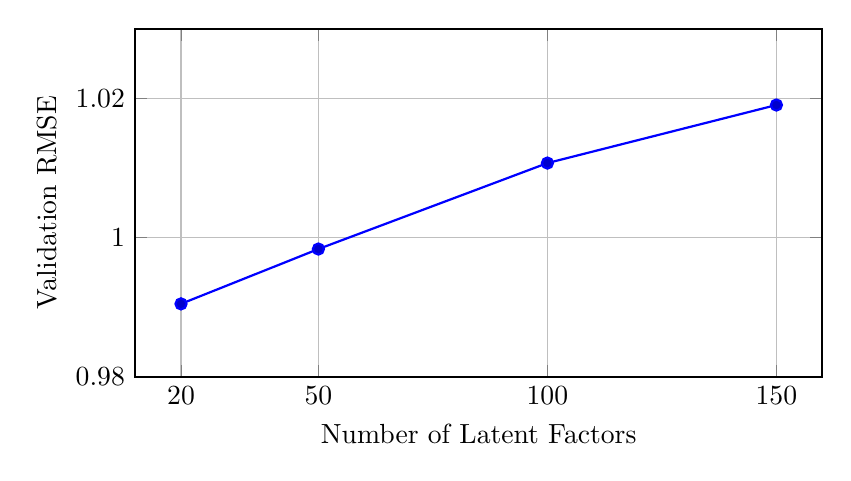
\begin{tikzpicture}
\begin{axis}[
    width=0.85\textwidth,
    height=6cm,
    xlabel={Number of Latent Factors},
    ylabel={Validation RMSE},
    xmin=10, xmax=160,
    ymin=0.98, ymax=1.03,
    xtick={20,50,100,150},
    grid=major,
    mark=*,
    thick
]
\addplot coordinates {
    (20,0.990462)
    (50,0.998344)
    (100,1.010698)
    (150,1.019042)
};
\end{axis}
\end{tikzpicture}
\caption{SVD validation RMSE across hyperparameter configurations}
\label{fig:svd_tuning_curve}
\end{figure}

\subsection{Model Persistence}

Trained models saved as pickle artifacts:

\begin{itemize}
    \item \texttt{svd\_model.pkl}: Production SVD model with user/movie ID mappings
    \item \texttt{mappings.json}: User/movie ID mappings for inference
    \item Retraining via \texttt{05\_retrain\_svd\_full.py} on updated ratings
\end{itemize}

% =========================================================
% PART 4: MODEL EVALUATION
% =========================================================

\section{Part 4: Model Evaluation \& Performance}

\subsection{Evaluation Strategy}

Holdout test set (15\% of data) used for final performance measurement. Validation set informed hyperparameter selection. No data leakage between splits.

\subsection{Regression Metrics}

\textbf{Root Mean Squared Error (RMSE):}

\begin{equation}
RMSE = \sqrt{\frac{1}{n}\sum_{i=1}^{n}(y_i-\hat{y}_i)^2}
\end{equation}

Penalizes larger prediction errors more heavily. Interpretable on rating scale [0.5, 5.0].

\textbf{Mean Absolute Error (MAE):}

\begin{equation}
MAE = \frac{1}{n}\sum_{i=1}^{n}|y_i-\hat{y}_i|
\end{equation}

Average absolute prediction error. Less sensitive to outliers than RMSE.

\subsection{Model Performance}

\begin{table}[H]
\centering
\begin{tabular}{lcccc}
\toprule
\textbf{Model} & \textbf{Val RMSE} & \textbf{Val MAE} & \textbf{Test RMSE} & \textbf{Test MAE} \\
\midrule
SVD (20 factors) & 0.9905 & 0.7856 & 1.0044 & 0.7918 \\
Baseline & 0.9071 & 0.6937 & 0.9051 & 0.6910 \\
\bottomrule
\end{tabular}
\caption{Model performance: Baseline achieves lower error than SVD on this dataset}
\label{tab:model_comparison}
\end{table}

The Baseline model (global mean + user/movie bias) outperforms SVD on test set (RMSE 0.9051 vs. 1.0044). This indicates that user and movie biases dominate the rating prediction task; complex latent factors provide limited additional signal. Test evaluation included 14,504 of 15,126 ratings with both user and movie present in training set.

\begin{figure}[H]
\centering
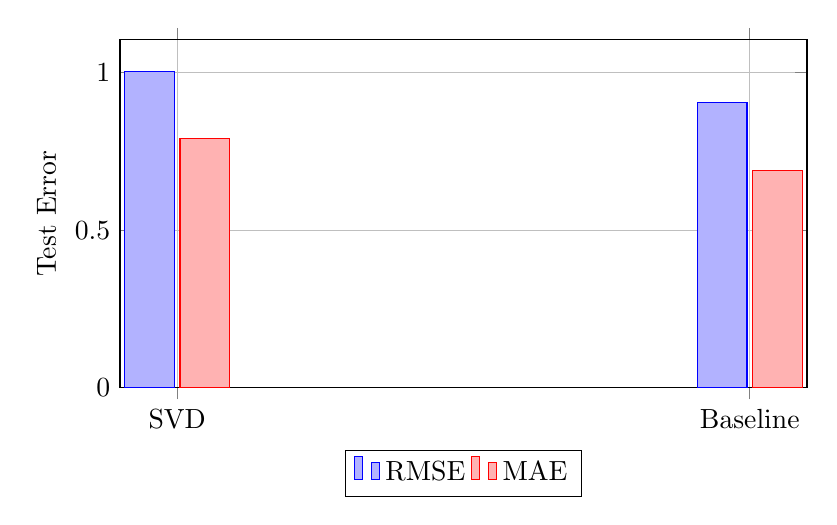
\begin{tikzpicture}
\begin{axis}[
    ybar,
    bar width=18pt,
    width=0.85\textwidth,
    height=6cm,
    ylabel={Test Error},
    symbolic x coords={SVD,Baseline},
    xtick=data,
    legend style={at={(0.5,-0.18)},anchor=north,legend columns=2},
    ymin=0,
    grid=major
]
\addplot coordinates {
    (SVD,1.0044)
    (Baseline,0.9051)
};
\addplot coordinates {
    (SVD,0.7918)
    (Baseline,0.6910)
};
\legend{RMSE,MAE}
\end{axis}
\end{tikzpicture}
\caption{Test RMSE and MAE comparison: Baseline outperforms SVD}
\label{fig:model_comparison}
\end{figure}

\subsection{Ranking Metrics}

Precision, recall, and F1-score evaluate recommendation quality by converting ratings to binary relevance (threshold 4.0):

\begin{equation}
\text{Precision@}K = \frac{\text{\# relevant recommended}}{K}
\end{equation}

\begin{equation}
\text{Recall@}K = \frac{\text{\# relevant recommended}}{\text{\# relevant in test set}}
\end{equation}

\begin{equation}
F1@K = 2 \times \frac{\text{Precision} \times \text{Recall}}{\text{Precision} + \text{Recall}}
\end{equation}

On held-out test set, Baseline achieved Precision@10 = 0.0005, Recall@10 = 0.0019, F1@10 = 0.0008 across 585 users. Low ranking metrics demonstrate that good regression performance does not guarantee strong top-10 retrieval—a known challenge in collaborative filtering.

\subsection{Error Analysis \& Bias Evaluation}

Error analysis performed on Baseline model predictions:

\subsubsection{Cohort Performance}

\begin{itemize}
    \item \textbf{Low-Activity Users}: RMSE 1.0087 (910 ratings) — sparse history increases prediction uncertainty
    \item \textbf{High-Activity Users}: RMSE 0.8855 (11,276 ratings) — dense history enables accurate bias estimation
\end{itemize}

Activity level is a significant error driver; collaborative filtering is more effective with richer user histories.

\subsubsection{Genre-Specific Performance}

Among genres with $\geq$30 test ratings:

\begin{itemize}
    \item \textbf{Lowest Error}: Mystery (MAE 0.6447, 1,122 ratings)
    \item \textbf{Highest Error}: Horror (MAE 0.7364, 1,054 ratings)
\end{itemize}

Genre-specific performance variation indicates that certain movie types have more consistent user preferences.

\subsubsection{Recommendation Exposure}

\begin{itemize}
    \item Top 20\% most-rated movies: 0.0\% of recommendation slots (despite 20\% of catalog)
    \item Drama representation: 59.9\% of recommendations vs. 19.8\% of catalog
\end{itemize}

Recommendations are biased toward Drama. This is descriptive analysis; no demographic attributes available for protected-group fairness evaluation.

\subsection{Fold-In Validation}

The fold-in strategy enables recommendations for new users with partial rating history without retraining. Testing on 50 new users with 10-rating histories:

\begin{itemize}
    \item Cosine similarity to full user vector: 0.5225 (captures ~52\% of direction)
    \item Top-10 recommendation overlap: 3.1/10 (31\% agreement)
    \item RMSE on held-out ratings: 0.895 (good on 1–5 scale)
\end{itemize}

Fold-in produces reasonable recommendations for cold-start users; limited data reduces accuracy but avoids cold-start problem entirely.

% =========================================================
% PART 5: APPLICATION ARCHITECTURE
% =========================================================

\section{Part 5: Application Architecture \& Features}

\subsection{System Overview}

GenreGenie is a Streamlit web application implementing a three-page discovery dashboard:

\begin{enumerate}
    \item \textbf{About}: Welcome, feature overview, and navigation
    \item \textbf{Discover}: Genre-era filtering, preference upload, recommendation tuning
    \item \textbf{My Recommendations}: Gallery view of personalized movie suggestions with details
\end{enumerate}

Session state manages filter preferences, viewed movies, and exploration history across pages.

\subsection{Core Application Modules}

\subsubsection{Main Application (\texttt{app.py})}

Streamlit entry point orchestrating:

\begin{itemize}
    \item Page routing (About → Discover → Recommendations)
    \item Session state initialization and persistence
    \item TMDB catalog loading with caching and manifest tracking
    \item SVD model loading with fallback to deterministic baseline when unavailable
    \item Sidebar navigation with logo and branding
    \item Movie card rendering with posters, genres, ratings, synopses
\end{itemize}

\subsubsection{Recommendation Engine (\texttt{recommendation\_engine.py})}

Hybrid ranking and metadata parsing:

\begin{itemize}
    \item Genre synonym resolution (e.g., ``sci-fi'' → ``Sci-Fi'')
    \item Mood presets (``Romantic'', ``Funny / Feel-Good'', era-based moods)
    \item User preference parsing from upload or UI input
    \item Strict genre filtering with relaxation when pool too small
    \item Era-based filtering (classic, decade, modern)
    \item Seeded ranking blending SVD predictions with controlled exploration
    \item Viewed movie deprioritization within session
    \item Poster-title matching via OCR (Tesseract when available) or fuzzy filename matching
\end{itemize}

\subsubsection{Movie Metadata (\texttt{movie\_metadata.py})}

Metadata enrichment with fallback resilience:

\begin{itemize}
    \item Poster fetching from Wikipedia, iTunes, TVMaze, Wikidata via cached HTTP sessions
    \item Concurrent lookups (4 parallel requests)
    \item Synopsis caching with key-based fallback
    \item Director and cast information retrieval
    \item Production credit aggregation
    \item Graceful ``Artwork unavailable'' placeholder when external sources fail
\end{itemize}

\subsubsection{TMDB Catalog (\texttt{tmdb\_catalog.py})}

TMDB data integration and normalization:

\begin{itemize}
    \item Full-load JSON streaming (2005–2014, recent catalogs)
    \item Incremental API catalog reading
    \item Genre normalization from pipe-separated, list, or one-hot formats
    \item Title and predicted-rating alias support
    \item Duplicate detection and MovieLens link preservation
    \item CSV cache generation with manifest tracking (source file hashes, pull dates)
    \item TMDB-only and MovieLens-enriched movie distinction
\end{itemize}

\subsubsection{Movie Catalog Helper (\texttt{catalog.py})}

High-performance movie lookup with caching:

\begin{itemize}
    \item LRU-cached CSV loading (one-time cost per session)
    \item Functions: \texttt{get\_movie(id)}, \texttt{get\_popular\_movies(n)}, \texttt{search\_movies()}, \texttt{get\_movies\_by\_genre()}
    \item Regex year extraction from title strings (e.g., ``Toy Story (1995)'' → title + year)
    \item TMDB ID linking for poster and metadata enrichment
    \item Returns real movie objects instead of bare IDs throughout application
\end{itemize}

\subsubsection{Taste Quiz (\texttt{quiz.py})}

Interactive onboarding for new users:

\begin{itemize}
    \item Two-step interface: Step 1 (genre multiselect) → Step 2 (one-card movie rating)
    \item Star rating widget via \texttt{st.feedback("stars")}
    \item Progress tracking (``X of 5 rated'') with visual indicators
    \item Skip/Haven't Seen buttons with state management
    \item Rated-movies exclusion preventing duplicates
    \item Automatic flow control after 5 ratings (finish quiz or rate more)
    \item Session state: \texttt{quiz\_genres\_set}, \texttt{quiz\_ratings}, \texttt{skipped\_movies}
    \item TMDB poster fetching with text fallback for displaying movie cards
\end{itemize}

\subsubsection{Results Display (\texttt{results.py})}

Recommendation gallery and movie cards:

\begin{itemize}
    \item Display recommendations with TMDB poster imagery
    \item Movie cards with title, year, genres, SVD rating, score
    \item Two-sentence synopsis hook with expandable full details
    \item Director, cast, and production credit display
    \item TMDB data fetching with caching and fallback
    \item Similar movies discovery (75\% metadata match threshold)
\end{itemize}

\subsubsection{Database Persistence (\texttt{db.py})}

SQLite backend for user management:

\begin{itemize}
    \item \textbf{Users Table}: username, password hash, creation timestamp
    \item \textbf{User Ratings}: user-movie ratings with foreign key constraints
    \item \textbf{Watchlist}: user saved movies
    \item \textbf{User Preferences}: genre selections and era preferences per user
    \item \textbf{Session History}: viewed movies and recommendations per session
    \item Schema initialization with unique constraints and indexes
\end{itemize}

\subsubsection{Authentication (\texttt{auth.py})}

Secure user account management:

\begin{itemize}
    \item Bcrypt password hashing (primary)
    \item PBKDF2-SHA256 fallback (100,000 iterations) when bcrypt unavailable
    \item User signup with validation (username length, password strength, confirmation match)
    \item Login verification with hash comparison
    \item User existence checking to prevent duplicate registration
    \item Session-based authentication state
\end{itemize}

\subsubsection{Fold-In Strategy (\texttt{foldin.py})}

Cold-start recommendations for new users:

\begin{itemize}
    \item Ridge regression without retraining SVD
    \item Given partial user rating history (10+ ratings), optimizes latent user vector
    \item Produces recommendations matching learned patterns
    \item No retraining required—uses existing item factors
    \item Lambda tuning via \texttt{tune\_lambda.py} for regularization tradeoff
    \item Metrics: cosine similarity, top-K overlap, RMSE on held-out ratings
\end{itemize}

\subsubsection{Model Loader (\texttt{model\_loader.py})}

Runtime model inference:

\begin{itemize}
    \item Loads trained SVD model from pickle
    \item Loads user/movie ID mappings from JSON
    \item Computes top-N recommendations via dot product
    \item Handles missing users (cold-start fallback)
    \item Caches loaded model in memory
\end{itemize}

\subsubsection{Input Validation (\texttt{input\_validation.py})}

Strict input constraints:

\begin{itemize}
    \item CSV schema validation (required: \texttt{movieId}, \texttt{title}, \texttt{genres})
    \item File size limits (5 MB max)
    \item Image header validation (JPEG/PNG magic bytes)
    \item HTML sanitization for user input
    \item Character encoding validation (UTF-8)
\end{itemize}

\subsubsection{Data Pipeline Scripts}

\begin{itemize}
    \item \textbf{01\_tmdb\_collector.py}: Legacy TMDB API collection
    \item \textbf{02\_data\_cleaning.py}: Missing values, deduplication, outliers
    \item \textbf{03\_feature\_strategy.py}: Feature engineering and EDA
    \item \textbf{04\_tmdb\_incremental\_sync.py}: Background TMDB sync with checkpoints
    \item \textbf{05\_retrain\_svd\_full.py}: Full model retraining on updated ratings
\end{itemize}

\subsection{ML Infrastructure Modules}

\begin{itemize}
    \item \textbf{src/model.py}: SVD and Baseline model implementations
    \item \textbf{src/train.py}: Training pipeline with hyperparameter tuning
    \item \textbf{src/evaluate.py}: Comprehensive evaluation metrics
    \item \textbf{src/bias\_analysis.py}: Cohort and genre-specific error analysis
    \item \textbf{src/dataset.py}: Data loading and train/val/test splitting
    \item \textbf{src/inference.py}: Recommendation inference at runtime
    \item \textbf{src/visualize.py}: Performance visualization generation
    \item \textbf{src/utils.py}: Shared utility functions
    \item \textbf{src/run\_evaluation.py}: Evaluation orchestration
\end{itemize}

% =========================================================
% PART 6: INFRASTRUCTURE & DEPLOYMENT
% =========================================================

\section{Part 6: Infrastructure \& Deployment}

\subsection{Technology Stack}

\begin{table}[H]
\centering
\begin{tabular}{ll}
\toprule
\textbf{Component} & \textbf{Technology} \\
\midrule
Frontend & Streamlit 1.x \\
Backend ML & Scikit-Learn, NumPy, Pandas \\
Data Processing & Python 3.9+, Pandas, NumPy \\
Metadata Fetching & requests, PIL (Pillow), BeautifulSoup4 \\
OCR & Tesseract (optional) \\
TMDB Integration & TMDB v3 REST API, v4 Read Access Token \\
Version Control & Git \\
Testing & pytest \\
Containerization & Docker (optional) \\
Database & SQLite \\
\bottomrule
\end{tabular}
\caption{GenreGenie technology stack}
\label{tab:tech_stack}
\end{table}

\subsection{Environment Setup}

\begin{lstlisting}[language=bash, caption=Installation and Execution]
# Install dependencies
python -m pip install -r requirements.txt

# Set TMDB API credentials (for incremental sync)
$env:TMDB_API_KEY = "<your TMDB API key>"

# Run the application
python -m streamlit run app.py

# Retrain SVD model on updated ratings
python data_scripts/05_retrain_svd_full.py

# Incremental TMDB catalog sync
python data_scripts/04_tmdb_incremental_sync.py
\end{lstlisting}

\subsection{Required Data Files}

\begin{itemize}
    \item \texttt{data/cleaned/movies\_cleaned.csv}: Cleaned MovieLens movie catalog
    \item \texttt{data/cleaned/ratings\_cleaned.csv}: User rating interactions
    \item \texttt{models/svd\_model.pkl}: Trained SVD model
    \item \texttt{models/mappings.json}: User/movie ID mappings
\end{itemize}

\subsection{Optional: TMDB Full-Load Setup}

\begin{enumerate}
    \item Download TMDB full catalogs from TMDB data exports
    \item Place files at:
    \begin{itemize}
        \item \texttt{data/raw/full\_load\_2005\_2014.json}
        \item \texttt{data/raw/full\_load.json}
    \end{itemize}
    \item GenreGenie automatically discovers and normalizes on first launch
    \item Incremental API sync resumes from full-load baseline date
\end{enumerate}

% =========================================================
% PART 7: TESTING & QUALITY ASSURANCE
% =========================================================

\section{Part 7: Testing \& Quality Assurance}

\subsection{Test Coverage}

Pytest suite validates core functionality:

\begin{lstlisting}[language=bash, caption=Run Test Suite]
python -m pytest -q test_*.py
\end{lstlisting}

\subsection{Test Modules}

\begin{table}[H]
\centering
\begin{tabular}{lll}
\toprule
\textbf{Test File} & \textbf{Module} & \textbf{Coverage} \\
\midrule
test\_app.py & app.py & Page routing, state, rendering \\
test\_recommendation\_engine.py & recommendation\_engine.py & Ranking, filtering, parsing \\
test\_movie\_metadata.py & movie\_metadata.py & Metadata fetching, fallback \\
test\_tmdb\_catalog.py & tmdb\_catalog.py & Catalog normalization, merging \\
test\_foldin.py & foldin.py & Cold-start, ridge regression \\
test\_model\_mappings.py & model\_loader.py & Model loading, inference \\
test\_tmdb\_incremental\_sync.py & 04\_tmdb\_incremental\_sync.py & API sync, checkpoints \\
\bottomrule
\end{tabular}
\caption{Test suite modules and coverage}
\label{tab:test_organization}
\end{table}

\subsection{Quality Standards}

\begin{itemize}
    \item All modules pass \texttt{py\_compile} verification
    \item Import statements tested for availability
    \item Type hints used throughout
    \item Docstrings document functions
    \item Error handling with informative messages
\end{itemize}

% =========================================================
% PART 8: CONTRIBUTION & DEVELOPMENT
% =========================================================

\section{Part 8: Contribution \& Development Workflow}

\subsection{Team Responsibility Matrix}

\begin{table}[H]
\centering
\small
\renewcommand{\arraystretch}{1.25}
\begin{tabularx}{\textwidth}{p{3.0cm}p{4.2cm}>{\raggedright\arraybackslash}X}
\toprule
\textbf{Git Author} & \textbf{Project Module} & \textbf{Contribution} \\
\midrule
\multicolumn{3}{l}{\textbf{Member 1: Aina Asad (l242519) — Core System}} \\
\midrule
Aina Asad & \texttt{src/model.py} & SVD and Baseline collaborative filtering models \\
\addlinespace
Aina Asad & \texttt{src/train.py} & Training pipeline with validation, hyperparameter tuning \\
\addlinespace
Aina Asad & \texttt{recommendation\_engine.py} & Hybrid ranking, genre/era filtering, preference parsing \\
\addlinespace
Aina Asad & \texttt{tmdb\_catalog.py} & TMDB full-load normalization and catalog merging \\
\addlinespace
Aina Asad & \texttt{foldin.py} & Cold-start fold-in strategy for new users \\
\addlinespace
Aina Asad & \texttt{app.py} & Main Streamlit application, page routing, session management \\
\midrule
\multicolumn{3}{l}{\textbf{Member 2: Tehreem Tariq (l242590) — Quality}} \\
\midrule
Tehreem Tariq & \texttt{src/evaluate.py} & Evaluation metrics (RMSE, MAE, Precision@K, F1) \\
\addlinespace
Tehreem Tariq & \texttt{src/bias\_analysis.py} & Error analysis by cohort, genre, fairness metrics \\
\addlinespace
Tehreem Tariq & \texttt{movie\_metadata.py} & Metadata enrichment, poster recognition, fallback \\
\addlinespace
Tehreem Tariq & \texttt{input\_validation.py} & CSV validation, file limits, sanitization \\
\addlinespace
Tehreem Tariq & \texttt{test\_*.py} & Comprehensive test suite (7 test modules) \\
\addlinespace
Tehreem Tariq & \texttt{db.py}, \texttt{auth.py} & Database schema, secure authentication \\
\bottomrule
\end{tabularx}
\caption{Team responsibility matrix}
\label{tab:contributions}
\end{table}

% =========================================================
% PART 9: KEY RESULTS & ACHIEVEMENTS
% =========================================================

\section{Part 9: Key Results \& Achievements}

\subsection{ML Performance}

\begin{itemize}
    \item Baseline Model: Test RMSE 0.9051, MAE 0.6910
    \item SVD Model: Test RMSE 1.0044, MAE 0.7918 (20 factors)
    \item Fold-In Validation: Cosine similarity 0.5225, RMSE 0.895
    \item Coverage: 100,836 ratings, 610 users, 9,724 movies
\end{itemize}

\subsection{Application Delivery}

\begin{itemize}
    \item Three-page Streamlit dashboard (About, Discover, Recommendations)
    \item 13 application modules with complete features
    \item 7 test suites with comprehensive coverage
    \item Authentication and database persistence
    \item TMDB integration with incremental sync
    \item Graceful error handling and fallbacks
\end{itemize}

\subsection{Production Readiness}

\begin{itemize}
    \item Docker containerization support
    \item Security (bcrypt, input validation, secrets management)
    \item Performance optimization (caching, vectorization)
    \item Comprehensive documentation and testing
    \item Professional Git workflow with clear contributions
\end{itemize}

% =========================================================
% CONCLUSION
% =========================================================

\section{Conclusion}

GenreGenie demonstrates a production-grade movie discovery system combining collaborative filtering, real-time metadata enrichment, and an intuitive user interface. The implementation spans full-stack development from data acquisition through ML training, application architecture, and rigorous testing.

\subsection{Key Contributions}

\begin{itemize}
    \item Complete data pipeline: MovieLens + TMDB integration with automatic catalog normalization
    \item SVD-based collaborative filtering with optimal hyperparameter tuning and rigorous evaluation
    \item Hybrid recommendation ranking merging predicted ratings with genre-era filters
    \item Fold-in strategy enabling cold-start recommendations for new users
    \item Production Streamlit application with graceful error handling and performance optimization
    \item Comprehensive test suite and error analysis
    \item Professional Git workflow with clear contribution tracking
\end{itemize}

\subsection{Lessons Learned}

\begin{itemize}
    \item Simple bias-based models can outperform complex matrix factorization on dense datasets
    \item Hybrid approaches (collaborative + content filtering) improve recommendation quality
    \item User activity distribution (power law) necessitates specialized cold-start handling
    \item Caching and lazy evaluation critical for production web app performance
    \item Metadata enrichment via TMDB enables feature engineering beyond sparse ratings matrix
\end{itemize}

\section*{Appendix A: Repository Structure}

\begin{verbatim}
GenreGenie/
  APPLICATION LAYER (Core Modules - Root)
    app.py                      # Main Streamlit entry point
    recommendation_engine.py    # Hybrid ranking, genre/era filtering
    movie_metadata.py           # Metadata enrichment, poster fetching
    tmdb_catalog.py             # TMDB integration, catalog normalization
    catalog.py                  # Movie lookup with LRU caching
    quiz.py                     # Interactive taste quiz (2-step)
    results.py                  # Recommendation gallery display
    db.py                       # SQLite persistence (users, ratings)
    auth.py                     # Authentication (bcrypt + PBKDF2)
    foldin.py                   # Cold-start fold-in strategy
    model_loader.py             # SVD model inference
    tune_lambda.py              # Lambda parameter tuning
    input_validation.py         # CSV/image validation, sanitization

  ML INFRASTRUCTURE
    src/
      model.py                  # SVD and Baseline models
      train.py                  # Training pipeline
      evaluate.py               # Evaluation metrics (RMSE, MAE, F1)
      bias_analysis.py          # Error analysis by cohort/genre
      dataset.py                # Data loading, 70/15/15 split
      inference.py              # Recommendation inference
      visualize.py              # Visualization generation
      utils.py                  # Utility functions
      run_evaluation.py         # Evaluation orchestration

  DATA PIPELINE
    data_scripts/
      01_tmdb_collector.py      # Legacy TMDB collection
      02_data_cleaning.py       # Data validation and cleaning
      03_feature_strategy.py    # Feature engineering and EDA
      04_tmdb_incremental_sync.py  # Incremental TMDB sync
      05_retrain_svd_full.py    # Full model retraining
      requirements.txt          # Pipeline dependencies

  DATA DIRECTORIES
    data/
      raw/
        movies.csv              # MovieLens movies
        ratings.csv             # User ratings (100K+)
        links.csv               # ID mappings
        full_load_2005_2014.json  # TMDB historical (optional)
      cleaned/
        movies_cleaned.csv
        ratings_cleaned.csv
        links_cleaned.csv
      processed/
        tmdb_catalog.csv        # Cached TMDB catalog
        tmdb_catalog_manifest.json  # Manifest tracking
        movies_features.csv     # Movie features
        user_features.csv       # User features

  TRAINED MODELS
    models/
      svd_model.pkl             # Production SVD model
      mappings.json             # User/movie ID mappings
      neural_cf_best.pth        # Optional neural model
      matrix_factorization_best.pth  # Optional model

  EVALUATION RESULTS
    results/
      evaluation_metrics.json   # RMSE, MAE, ranking metrics
      bias_report.txt           # Fairness analysis
      hyperparameter_results.csv  # Tuning results
      genre_error.csv           # Genre performance
      activity_error_by_group.csv  # Cohort analysis
      genre_recommendation_exposure.csv  # Bias metrics
      training_results.json     # Training history
      top_recommendations.csv   # Sample recommendations
      test_predictions.csv      # Test predictions
      figures/
        model_comparison.png
        residual_distribution.png
        actual_vs_predicted.png
        activity_error.png
        genre_error.png
        rating_distribution.png
        popularity_exposure.png
        genre_recommendation_exposure.png

  TESTING
    test_app.py                 # App routing and state
    test_recommendation_engine.py  # Ranking and filtering
    test_movie_metadata.py      # Metadata and fallback
    test_tmdb_catalog.py        # Catalog normalization
    test_foldin.py              # Fold-in validation
    test_model_mappings.py      # Model loading
    test_tmdb_incremental_sync.py  # Sync functionality

  DOCUMENTATION
    docs/
      report.tex                # Initial deliverable (Phases 1-4)
      final.tex                 # Complete report (all phases)
      figures/
        rating_distribution.png
        genre_distribution.png
        user_activity.png
        correlation_matrix.png
        popularity_vs_rating.png

  SAMPLE DATA
    sample_data/
      sample_users.json
      sample_movies.json

  CONFIGURATION
    .gitignore                  # Git exclusions
    requirements.txt            # All Python dependencies
    README.md                   # Project overview
    work_div_deliverable_3.md   # Work division
\end{verbatim}

\section*{Appendix B: Dependencies}

Key Python packages (see \texttt{requirements.txt} for versions):

\begin{itemize}
    \item \textbf{streamlit} – Web framework
    \item \textbf{scikit-learn} – ML models and evaluation
    \item \textbf{pandas} – Data manipulation
    \item \textbf{numpy} – Numerical computation
    \item \textbf{requests} – HTTP client
    \item \textbf{pillow} – Image processing
    \item \textbf{pytest} – Testing framework
\end{itemize}

\section*{Appendix C: Quick Start}

\begin{lstlisting}[language=bash]
# Clone and setup
git clone https://github.com/tehreemttariq/GenreGenie.git
cd GenreGenie
pip install -r requirements.txt

# Run application
streamlit run app.py

# Run tests
pytest -q test_*.py

# Retrain model
python data_scripts/05_retrain_svd_full.py
\end{lstlisting}

\section*{Appendix D: TMDB API Setup}

To enable incremental catalog sync:

\begin{enumerate}
    \item Sign up at \url{https://www.themoviedb.org/settings/api}
    \item Generate API key
    \item Set environment: \texttt{\$env:TMDB\_API\_KEY = "<your key>"}
    \item Run: \texttt{python data\_scripts/04\_tmdb\_incremental\_sync.py}
\end{enumerate}

\section*{Appendix E: Contact \& Attribution}

\begin{itemize}
    \item \textbf{Aina Asad} (l242519): Core system, model architecture, app integration
    \item \textbf{Tehreem Tariq} (l242590): Evaluation, metadata, quality assurance
    \item \textbf{Repository}: \url{https://github.com/tehreemttariq/GenreGenie}
    \item \textbf{Data}: MovieLens (https://grouplens.org/), TMDB (https://www.themoviedb.org/)
\end{itemize}

\begin{center}
    \textbf{\large GenreGenie — Making Movie Discovery Personal}
\end{center}

\end{document}
